\section{Research Plan}
	It is apparent from the literature that operators and amplitude expressions in tensors in quantum chemistry have some compact format that can be taken advantage %of as the dimension of a system increases, ie number of electrons. 
	It is the goal for this research to apply tensor decomposition algorithms, which make use of modern computational architecture, to reduce computational complexity of correlation methods based on MBPT, CC, and CC-R12 methods. 
	%modern computational architecture scaling tensor decomposition algorithms to reduce scaling of correlation methods based on MBPT, CC and CC-R12 methods. 
	%THC is quantum chemistries first step into utilizing the structure of tensor decompositions to reduce storage requirements without arbitrary truncation based on practiced thresholds.
	%CP and Tucker decompositions dissect the character from the full set of vectors which span the tensor space, unlike the truncated SVD or eigenvalue decomposition. 
	CP and Tucker decompositions encode the behavior of every element in a given tensor into a set of factor matrices with reduced storage requirements. 
	%In PNO and OSV methods virtual set domain truncation is based on either a occupation number or the diagonal MP2 amplitude threshold and rank is reduced by removing information.  
	While truncation methods based on an eigenvalue, occupation number, or diagonal MP2 amplitudes discard information deemed unnecessary. Implementing tensor decompositions, instead of these truncation methods, to reduce storage requirements allows for data compression without significantly loss of information. Figure 4 and 5 show how memory requirements of canonical tensors in quantum chemistry, such as the TEIs, can be significantly reduced with little cost in accuracy.
	%Changing these rank reduction methods to tensor decompositions would allow for data compression without loss of information. These new rank reductions methods c assist in the calculation of molecular properties where for example loss of even small valued vectors could have large contributions in derivative based response properties. 

		\begin{figure}
			\centering
				\begin{minipage}{.5\textwidth}
				  \centering
				  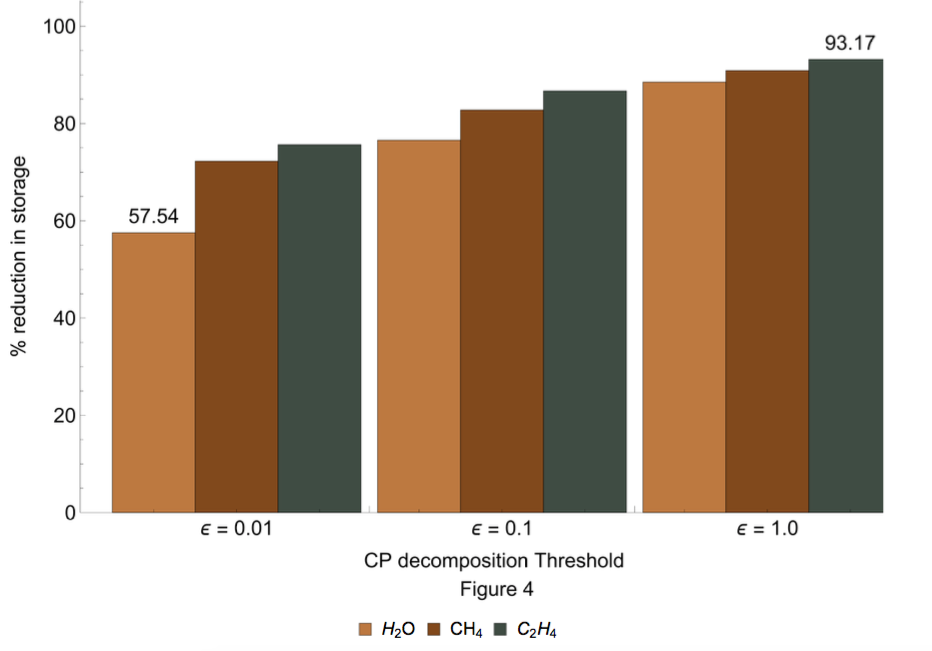
\includegraphics[width=1\linewidth]{./plots/Store}
				  %\captionof{figure}{Reduced storage requirements of TEI after CP decomposition }
				  \label{fig:Figure 4}
				\end{minipage}%
				\begin{minipage}{.5\textwidth}
				  \centering
				  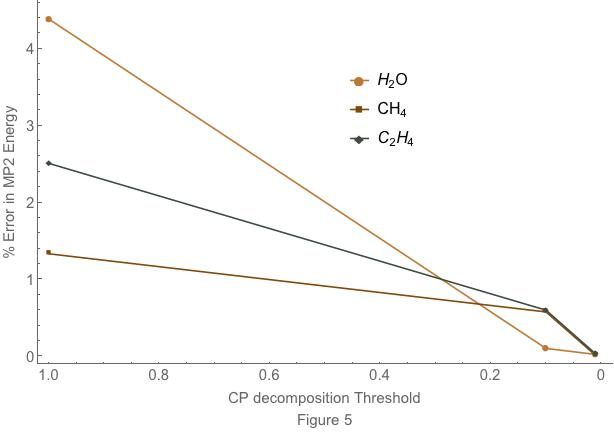
\includegraphics[width=1 \linewidth]{./plots/Energy}
				  \label{fig:Figure 5}
				\end{minipage}
				\caption{Reduced storage requirements of global AO TEI tensor after CP decomposition\\
				\textbf{Figure 5:} MP2 energy calculated using the CP decomposed global AO TEI methods presented by Benedikt et al\cite{Benedikt2011} compared to canonical closed-shell spin-restricted MP2 calculations.\\
				Following Benedikt's implementation the HF orbital energy denominator term was decomposed to a CP threshold of $\epsilon = .01$; Calculations on $\text{H}_2\text{O}$ and $\text{CH}_4$ were performed using a 6-31G* basis and calculations on $\text{C}_2\text{H}_4$ used a 6-31G basis}
		\end{figure}

	In order to reduce the computational demands of computing the CP decomposition modern mathematics turns to tensor compression.  Tensor compression techniques reduce computational bottleneck of large tensor using a smaller proxy tensor, which are then used to approximately the CP decomposition. Original methods to compute a tensor compression used the Tucker decomposition\cite{Bro1998,Lathauwer2000}. However, this approach requires the computation of an expensive singular value decomposition on each mode of a tensor. More recently, mathematicians have found that randomized tensor compression methods can achieve significant computational savings while producing near-optimal approximation quality\cite{Erichson2017}. Application of these compression methods, to tensors which are too either large to store in fast memory or are slow to converge to their optimal rank, will allow for reduced scale tensor algebra methods to be more reasonably applied to single reference quantum chemistry.

	Generally the tools in computational chemistry have limited application, such as CCSD(T) or CCSD-RI, because computational scaling and storage  requirements are unmanageably high.  Work presented by Benedikt et al\cite{Benedikt2011,Benedikt2013,Benedikt2013a,Benedikt2014} is the first step to understanding how to reformulate canonical many-body ab initio quantum mechanic equations into a decomposed tensor algebra framework.  Benedikt's ideas can be extended by work presented by Parrish et al\cite{Parrish2012}.  Using the CP decomposition on a form of DF TEI reduces the storage requirements of integral tensor while tensor algebra expressions reduce the operations required to calculate observables. This idea can be further extended to reduced scaling accurate molecular properties. For example using CADF work presented by Hollman et all\cite{Hollman2014}, one can compute "localized" analytical gradients of the TEIs where, either the gradients are decomposed during their computation or CADF third order tensors are first decomposed then analytical gradient expressions are calculated using tensor algebra expressions.  
	%Though, tensor decomposition methods to compress higher order amplitude expressions has not yet been explored by quantum chemistry. Tensor decompositions will also allow for method development in reduced scaling accurate molecular property investigation, where truncation based approaches can significant influence a property's value.
  %Application of CP decompositions to CADF will decouple electronic indices's from electronic density terms allowing one to calculate more simply HF exchange terms. %Hollman and co-authors CADF method reduced computational cost with less error th 

	In work originally presented by Alm{\"o}f\cite{Almlof1991} and later H{\"a}ser\
	\cite{Haser1992} it has been shown that the AO to MO integral transform step of perturbation methods, such as MP2 \cref{AO2MO}, can be simplified using a Laplace transform of the denominator term
		\begin{equation}\label{LP_MP2}
			D_{ijab} = \frac{1}{\epsilon_i + \epsilon_j - \epsilon_a - \epsilon_b} = \int e^{(\epsilon_i + \epsilon_j - \epsilon_a - \epsilon_b)t}dt
		\end{equation}
	from there the exponential term can be factored into the AO wavefuntion
		\begin{equation}
			\ket{\phi_i} = \ket{\phi_i}e^{-\epsilon_i t/2}
		\end{equation}
		\begin{equation}
			\ket{\phi_a} = \ket{\phi_a}e^{\epsilon_a t/2}
		\end{equation}
	Computationally the integral in \cref{LP_MP2} can be transformed to a finite sum
		\begin{equation}
			E_{MP2} = \sum_\alpha^\tau w_\alpha e_2^\alpha
		\end{equation}
	$e_2^\alpha$ is the weighted integral form of \cref{AO2MO} based on the difference in energy between $\epsilon_i$ or $\epsilon_a$ and $\epsilon_F$ the fermi level.  These integrals can be in AO basis or any non-canonical form.  Using tensor decomposition methods one can optimize the weighting coefficients and calculate more accurate quadrature points.  Laplace transform methods coupled with tensor decompositions to perturbation theories, such as CCSD(T) and CCSD(T)-R12, could reduce the storage and computational complexity of these methods allowing one to compute energy values of increasingly large molecules extremely accurately.